\documentclass[tikz,border=10pt]{standalone}
\usepackage{tikz}
\usetikzlibrary{arrows.meta, positioning, fit, backgrounds}
\begin{document}
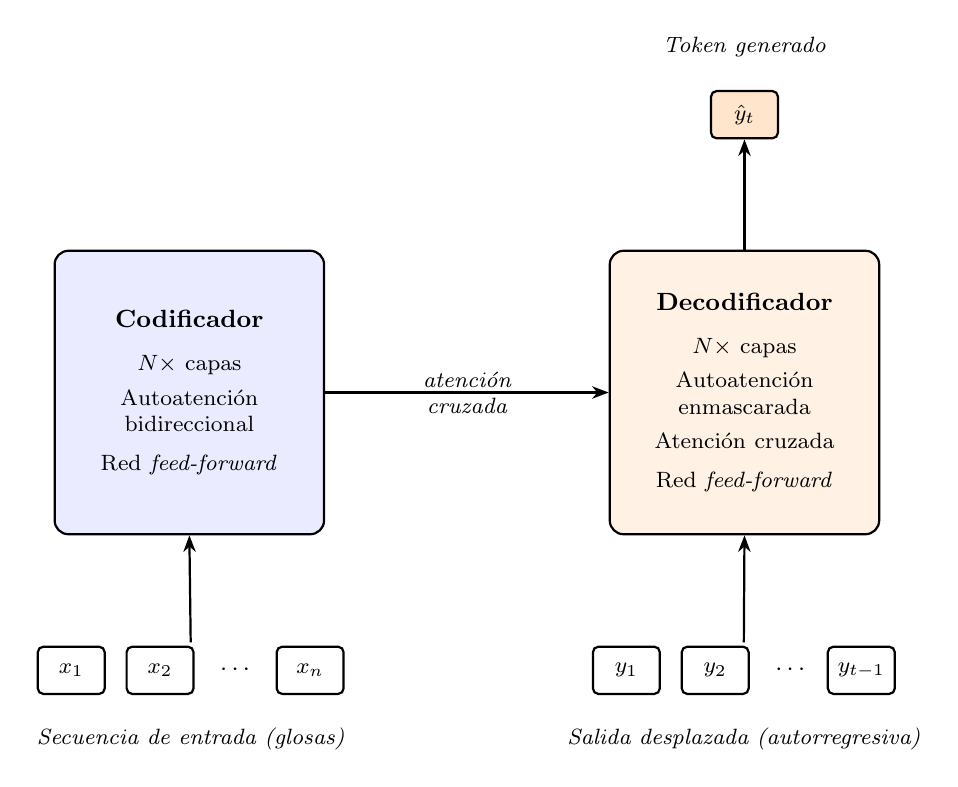
\begin{tikzpicture}[
    font=\small,
    stack/.style = {rounded corners=5pt, draw, thick, align=center,
                    text width=3.0cm, minimum height=3.6cm, inner sep=6pt},
    io/.style    = {draw, thick, rounded corners=2pt, align=center,
                    minimum width=0.85cm, minimum height=0.6cm, font=\footnotesize},
    arrow/.style = {-{Stealth[length=6pt]}, thick},
    lbl/.style   = {font=\footnotesize\itshape}
]

%% ── Bloques principales ─────────────────────────────────────────────────────
\node[stack, fill=blue!8] (enc) {\textbf{Codificador}\\[6pt]
        \footnotesize $N\times$ capas\\[3pt]
        \footnotesize Autoatención\\\footnotesize bidireccional\\[3pt]
        \footnotesize Red \textit{feed-forward}};

\node[stack, fill=orange!10, right=3.6cm of enc] (dec) {\textbf{Decodificador}\\[6pt]
        \footnotesize $N\times$ capas\\[3pt]
        \footnotesize Autoatención\\\footnotesize enmascarada\\[3pt]
        \footnotesize Atención cruzada\\[3pt]
        \footnotesize Red \textit{feed-forward}};

%% ── Atención cruzada (codificador → decodificador) ─────────────────────────
\draw[arrow] (enc.east) -- node[lbl, align=center]{atención\\cruzada} (dec.west);

%% ── Entrada del codificador ─────────────────────────────────────────────────
\node[io, below=1.4cm of enc.south, xshift=-1.5cm] (x1) {$x_1$};
\node[io, right=0.25cm of x1] (x2) {$x_2$};
\node[right=0.2cm of x2] (xdots) {$\cdots$};
\node[io, right=0.2cm of xdots] (xn) {$x_n$};
\node[fit=(x1)(xn), inner sep=1pt] (xgroup) {};
\draw[arrow] (xgroup.north) -- (enc.south);
\node[lbl, below=0.25cm of xgroup] {Secuencia de entrada (glosas)};

%% ── Entrada del decodificador (salida desplazada) ──────────────────────────
\node[io, below=1.4cm of dec.south, xshift=-1.5cm] (y1) {$y_1$};
\node[io, right=0.25cm of y1] (y2) {$y_2$};
\node[right=0.2cm of y2] (ydots) {$\cdots$};
\node[io, right=0.15cm of ydots] (yt) {$y_{t-1}$};
\node[fit=(y1)(yt), inner sep=1pt] (ygroup) {};
\draw[arrow] (ygroup.north) -- (dec.south);
\node[lbl, below=0.25cm of ygroup] {Salida desplazada (autorregresiva)};

%% ── Salida del decodificador ────────────────────────────────────────────────
\node[io, fill=orange!20, above=1.4cm of dec.north] (out) {$\hat{y}_t$};
\draw[arrow] (dec.north) -- (out.south);
\node[lbl, above=0.3cm of out] {Token generado};

\end{tikzpicture}
\end{document}
